\documentclass[a4paper]{book}
\usepackage{makeidx}
\usepackage{natbib}
\usepackage{graphicx}
\usepackage{multicol}
\usepackage{float}
\usepackage{listings}
\usepackage{color}
\usepackage{ifthen}
\usepackage[table]{xcolor}
\usepackage{textcomp}
\usepackage{alltt}
\usepackage{ifpdf}
\ifpdf
\usepackage[pdftex,
            pagebackref=true,
            colorlinks=true,
            linkcolor=blue,
            unicode
           ]{hyperref}
\else
\usepackage[ps2pdf,
            pagebackref=true,
            colorlinks=true,
            linkcolor=blue,
            unicode
           ]{hyperref}
\usepackage{pspicture}
\fi
\usepackage[utf8]{inputenc}
\usepackage[brazil]{babel}
\usepackage{mathptmx}
\usepackage[scaled=.90]{helvet}
\usepackage{courier}
\usepackage{sectsty}
\usepackage[titles]{tocloft}
\usepackage{doxygen}
\lstset{language=C++,inputencoding=utf8,basicstyle=\footnotesize,breaklines=true,breakatwhitespace=true,tabsize=8,numbers=left }
\makeindex
\setcounter{tocdepth}{3}
\renewcommand{\footrulewidth}{0.4pt}
\renewcommand{\familydefault}{\sfdefault}
\hfuzz=15pt
\setlength{\emergencystretch}{15pt}
\hbadness=750
\tolerance=750
\begin{document}
\hypersetup{pageanchor=false,citecolor=blue}
\begin{titlepage}
\vspace*{7cm}
\begin{center}
{\Large \-Testes do \-Sistema de \-Projetos dos \-Alunos }\\
\vspace*{1cm}
{\large \-Gerado por Doxygen 1.7.5.1}\\
\vspace*{0.5cm}
{\small Segunda, 10 de Outubro de 2011 17:09:31}\\
\end{center}
\end{titlepage}
\clearemptydoublepage
\pagenumbering{roman}
\tableofcontents
\clearemptydoublepage
\pagenumbering{arabic}
\hypersetup{pageanchor=true,citecolor=blue}
\chapter{\-Testes do \-Sistema de \-Projetos de \-Alunos}
\label{index}\hypertarget{index}{}\-Esse sistema realiza os testes dos tipos basicos definidos no \-Sistema de \-Projeto de \-Alunos. \-Para cada tipo basico realiza-\/se um teste usando um argumento valido e um invalido. 
\chapter{Índice dos \-Componentes}
\section{\-Hierarquia de classes}
\-Esta lista de heranças está organizada, dentro do possível, por ordem alfabética\-:\begin{DoxyCompactList}
\item \contentsline{section}{\-Cntr\-Int\-Navegacao}{\pageref{class_cntr_int_navegacao}}{}
\item \contentsline{section}{\-Codigo\-\_\-\-Fase}{\pageref{class_codigo___fase}}{}
\item \contentsline{section}{\-Codigo\-\_\-\-Modulo}{\pageref{class_codigo___modulo}}{}
\item \contentsline{section}{\-Codigo\-\_\-\-Projeto}{\pageref{class_codigo___projeto}}{}
\item \contentsline{section}{\-Data\-\_\-\-Inicio}{\pageref{class_data___inicio}}{}
\item \contentsline{section}{\-Data\-\_\-\-Termino}{\pageref{class_data___termino}}{}
\item \contentsline{section}{\-Fase}{\pageref{class_fase}}{}
\begin{DoxyCompactList}
\item \contentsline{section}{\-Stub\-Fase}{\pageref{class_stub_fase}}{}
\end{DoxyCompactList}
\item \contentsline{section}{\-Matricula}{\pageref{class_matricula}}{}
\item \contentsline{section}{\-Metrica}{\pageref{class_metrica}}{}
\begin{DoxyCompactList}
\item \contentsline{section}{\-Stub\-Metrica}{\pageref{class_stub_metrica}}{}
\end{DoxyCompactList}
\item \contentsline{section}{\-Modulo}{\pageref{class_modulo}}{}
\begin{DoxyCompactList}
\item \contentsline{section}{\-Stub\-Modulo}{\pageref{class_stub_modulo}}{}
\end{DoxyCompactList}
\item \contentsline{section}{\-Nome\-\_\-\-Arquivo}{\pageref{class_nome___arquivo}}{}
\item \contentsline{section}{\-Nota}{\pageref{class_nota}}{}
\item \contentsline{section}{\-Projeto}{\pageref{class_projeto}}{}
\begin{DoxyCompactList}
\item \contentsline{section}{\-Stub\-Projeto}{\pageref{class_stub_projeto}}{}
\end{DoxyCompactList}
\item \contentsline{section}{\-Protocolo\-Fase}{\pageref{class_protocolo_fase}}{}
\begin{DoxyCompactList}
\item \contentsline{section}{\-Stub\-Fase}{\pageref{class_stub_fase}}{}
\end{DoxyCompactList}
\item \contentsline{section}{\-Protocolo\-Int}{\pageref{class_protocolo_int}}{}
\begin{DoxyCompactList}
\item \contentsline{section}{\-Protocolo\-Int\-Fase}{\pageref{class_protocolo_int_fase}}{}
\begin{DoxyCompactList}
\item \contentsline{section}{\-Cntr\-Int\-Fase}{\pageref{class_cntr_int_fase}}{}
\end{DoxyCompactList}
\item \contentsline{section}{\-Protocolo\-Int\-Metrica}{\pageref{class_protocolo_int_metrica}}{}
\begin{DoxyCompactList}
\item \contentsline{section}{\-Cntr\-Int\-Metrica}{\pageref{class_cntr_int_metrica}}{}
\end{DoxyCompactList}
\item \contentsline{section}{\-Protocolo\-Int\-Modulo}{\pageref{class_protocolo_int_modulo}}{}
\begin{DoxyCompactList}
\item \contentsline{section}{\-Cntr\-Int\-Modulo}{\pageref{class_cntr_int_modulo}}{}
\end{DoxyCompactList}
\item \contentsline{section}{\-Protocolo\-Int\-Projeto}{\pageref{class_protocolo_int_projeto}}{}
\begin{DoxyCompactList}
\item \contentsline{section}{\-Cntr\-Int\-Projeto}{\pageref{class_cntr_int_projeto}}{}
\end{DoxyCompactList}
\end{DoxyCompactList}
\item \contentsline{section}{\-Protocolo\-Metrica}{\pageref{class_protocolo_metrica}}{}
\begin{DoxyCompactList}
\item \contentsline{section}{\-Stub\-Metrica}{\pageref{class_stub_metrica}}{}
\end{DoxyCompactList}
\item \contentsline{section}{\-Protocolo\-Modulo}{\pageref{class_protocolo_modulo}}{}
\begin{DoxyCompactList}
\item \contentsline{section}{\-Stub\-Modulo}{\pageref{class_stub_modulo}}{}
\end{DoxyCompactList}
\item \contentsline{section}{\-Protocolo\-Projeto}{\pageref{class_protocolo_projeto}}{}
\begin{DoxyCompactList}
\item \contentsline{section}{\-Stub\-Projeto}{\pageref{class_stub_projeto}}{}
\end{DoxyCompactList}
\item \contentsline{section}{\-Tamanho}{\pageref{class_tamanho}}{}
\item \contentsline{section}{\-Tempo}{\pageref{class_tempo}}{}
\end{DoxyCompactList}

\chapter{Índice dos \-Componentes}
\section{\-Lista de componentes}
\-Lista de classes, estruturas, uniões e interfaces com uma breve descrição\-:\begin{DoxyCompactList}
\item\contentsline{section}{\hyperlink{class_cntr_int_fase}{\-Cntr\-Int\-Fase} \\*\-Classe que representa a controladora de interacao \-Usuario/\-Fase }{\pageref{class_cntr_int_fase}}{}
\item\contentsline{section}{\hyperlink{class_cntr_int_metrica}{\-Cntr\-Int\-Metrica} \\*\-Classe que representa a controladora de interacao \-Usuario/\-Metrica }{\pageref{class_cntr_int_metrica}}{}
\item\contentsline{section}{\hyperlink{class_cntr_int_modulo}{\-Cntr\-Int\-Modulo} \\*\-Classe que representa a controladora de interacao \-Usuario/\-Modulo }{\pageref{class_cntr_int_modulo}}{}
\item\contentsline{section}{\hyperlink{class_cntr_int_navegacao}{\-Cntr\-Int\-Navegacao} \\*\-Classe que representa a controladora de interacao \-Usuario/\-Navegacao }{\pageref{class_cntr_int_navegacao}}{}
\item\contentsline{section}{\hyperlink{class_cntr_int_projeto}{\-Cntr\-Int\-Projeto} \\*\-Classe que representa a controladora de interacao \-Usuario/\-Projeto }{\pageref{class_cntr_int_projeto}}{}
\item\contentsline{section}{\hyperlink{class_cntr_l_n_fase}{\-Cntr\-L\-N\-Fase} \\*\-Classe que representa a controladora de logica de negocio relacionada as fases }{\pageref{class_cntr_l_n_fase}}{}
\item\contentsline{section}{\hyperlink{class_cntr_l_n_metrica}{\-Cntr\-L\-N\-Metrica} \\*\-Classe que representa a controladora de logica de negocio relacionada as metricas }{\pageref{class_cntr_l_n_metrica}}{}
\item\contentsline{section}{\hyperlink{class_cntr_l_n_modulo}{\-Cntr\-L\-N\-Modulo} \\*\-Classe que representa a controladora de logica de negocio relacionada aos modulos }{\pageref{class_cntr_l_n_modulo}}{}
\item\contentsline{section}{\hyperlink{class_cntr_l_n_projeto}{\-Cntr\-L\-N\-Projeto} \\*\-Classe que representa a controladora de logica de negocio relacionada aos projetos }{\pageref{class_cntr_l_n_projeto}}{}
\item\contentsline{section}{\hyperlink{class_cntr_persistencia}{\-Cntr\-Persistencia} \\*\-Classe que representa a \-Controladora de \-Persistencia }{\pageref{class_cntr_persistencia}}{}
\item\contentsline{section}{\hyperlink{class_codigo___fase}{\-Codigo\-\_\-\-Fase} \\*\-Classe que representa o dominio \hyperlink{class_codigo___fase}{\-Codigo\-\_\-\-Fase} }{\pageref{class_codigo___fase}}{}
\item\contentsline{section}{\hyperlink{class_codigo___modulo}{\-Codigo\-\_\-\-Modulo} \\*\-Classe que representa o dominio \hyperlink{class_codigo___modulo}{\-Codigo\-\_\-\-Modulo} }{\pageref{class_codigo___modulo}}{}
\item\contentsline{section}{\hyperlink{class_codigo___projeto}{\-Codigo\-\_\-\-Projeto} \\*\-Classe que representa o dominio \hyperlink{class_codigo___projeto}{\-Codigo\-\_\-\-Projeto} }{\pageref{class_codigo___projeto}}{}
\item\contentsline{section}{\hyperlink{class_comando_atualizar_fase}{\-Comando\-Atualizar\-Fase} \\*\-Classe que simula servicos da classe \hyperlink{class_protocolo_persistencia}{\-Protocolo\-Persistencia} }{\pageref{class_comando_atualizar_fase}}{}
\item\contentsline{section}{\hyperlink{class_comando_atualizar_modulo}{\-Comando\-Atualizar\-Modulo} \\*\-Classe que simula servicos da classe \hyperlink{class_protocolo_persistencia}{\-Protocolo\-Persistencia} }{\pageref{class_comando_atualizar_modulo}}{}
\item\contentsline{section}{\hyperlink{class_comando_atualizar_projeto}{\-Comando\-Atualizar\-Projeto} \\*\-Classe que simula servicos da classe \hyperlink{class_protocolo_persistencia}{\-Protocolo\-Persistencia} }{\pageref{class_comando_atualizar_projeto}}{}
\item\contentsline{section}{\hyperlink{class_comando_b_d}{\-Comando\-B\-D} \\*\-Classe que representa os \-Comandos do \-Bando de \-Dados }{\pageref{class_comando_b_d}}{}
\item\contentsline{section}{\hyperlink{class_comando_cadastrar_fase}{\-Comando\-Cadastrar\-Fase} \\*\-Classe que simula servicos da classe \hyperlink{class_protocolo_persistencia}{\-Protocolo\-Persistencia} }{\pageref{class_comando_cadastrar_fase}}{}
\item\contentsline{section}{\hyperlink{class_comando_cadastrar_modulo}{\-Comando\-Cadastrar\-Modulo} \\*\-Classe que simula servicos da classe \hyperlink{class_protocolo_persistencia}{\-Protocolo\-Persistencia} }{\pageref{class_comando_cadastrar_modulo}}{}
\item\contentsline{section}{\hyperlink{class_comando_cadastrar_projeto}{\-Comando\-Cadastrar\-Projeto} \\*\-Classe que simula servicos da classe \hyperlink{class_protocolo_persistencia}{\-Protocolo\-Persistencia} }{\pageref{class_comando_cadastrar_projeto}}{}
\item\contentsline{section}{\hyperlink{class_comando_nota}{\-Comando\-Nota} \\*\-Classe \hyperlink{class_comando_nota}{\-Comando\-Nota} herda a classe comando\-B\-D e prove servicos para calcular as notas }{\pageref{class_comando_nota}}{}
\item\contentsline{section}{\hyperlink{class_comando_numero_linhas}{\-Comando\-Numero\-Linhas} \\*\-Classe \hyperlink{class_comando_numero_linhas}{\-Comando\-Numero\-Linhas} herda a classe comando\-B\-D e prove servicos para calcular o numero de linhas }{\pageref{class_comando_numero_linhas}}{}
\item\contentsline{section}{\hyperlink{class_comando_pesquisar_fase}{\-Comando\-Pesquisar\-Fase} \\*\-Classe que simula servicos da classe \hyperlink{class_protocolo_persistencia}{\-Protocolo\-Persistencia} }{\pageref{class_comando_pesquisar_fase}}{}
\item\contentsline{section}{\hyperlink{class_comando_pesquisar_modulo}{\-Comando\-Pesquisar\-Modulo} \\*\-Classe que simula servicos da classe \hyperlink{class_protocolo_persistencia}{\-Protocolo\-Persistencia} }{\pageref{class_comando_pesquisar_modulo}}{}
\item\contentsline{section}{\hyperlink{class_comando_pesquisar_projeto}{\-Comando\-Pesquisar\-Projeto} \\*\-Classe que simula servicos da classe \hyperlink{class_protocolo_persistencia}{\-Protocolo\-Persistencia} }{\pageref{class_comando_pesquisar_projeto}}{}
\item\contentsline{section}{\hyperlink{class_comando_produtividade_media}{\-Comando\-Produtividade\-Media} \\*\-Classe \hyperlink{class_comando_produtividade_media}{\-Comando\-Produtividade\-Media} herda a classe comando\-B\-D e prove servicos para calcular a produtividade media }{\pageref{class_comando_produtividade_media}}{}
\item\contentsline{section}{\hyperlink{class_comando_produtividade_modulo}{\-Comando\-Produtividade\-Modulo} \\*\-Classe \hyperlink{class_comando_produtividade_modulo}{\-Comando\-Produtividade\-Modulo} herda a classe comando\-B\-D e prove servicos para calcular a produtividade do modulo }{\pageref{class_comando_produtividade_modulo}}{}
\item\contentsline{section}{\hyperlink{class_comando_produtividade_projeto}{\-Comando\-Produtividade\-Projeto} \\*\-Classe \hyperlink{class_comando_produtividade_projeto}{\-Comando\-Produtividade\-Projeto} herda a classe comando\-B\-D e prove servicos para calcular a produtividade do projeto }{\pageref{class_comando_produtividade_projeto}}{}
\item\contentsline{section}{\hyperlink{class_comando_remover_fase}{\-Comando\-Remover\-Fase} \\*\-Classe que simula servicos da classe \hyperlink{class_protocolo_persistencia}{\-Protocolo\-Persistencia} }{\pageref{class_comando_remover_fase}}{}
\item\contentsline{section}{\hyperlink{class_comando_remover_modulo}{\-Comando\-Remover\-Modulo} \\*\-Classe que simula servicos da classe \hyperlink{class_protocolo_persistencia}{\-Protocolo\-Persistencia} }{\pageref{class_comando_remover_modulo}}{}
\item\contentsline{section}{\hyperlink{class_comando_remover_projeto}{\-Comando\-Remover\-Projeto} \\*\-Classe que simula servicos da classe \hyperlink{class_protocolo_persistencia}{\-Protocolo\-Persistencia} }{\pageref{class_comando_remover_projeto}}{}
\item\contentsline{section}{\hyperlink{class_comandos_modulo}{\-Comandos\-Modulo} \\*\-Classe \hyperlink{class_comandos_modulo}{\-Comandos\-Modulo} herda a classe \-Comandos\-B\-D e prove servicos pros comandos de \-Modulos }{\pageref{class_comandos_modulo}}{}
\item\contentsline{section}{\hyperlink{class_comandos_projeto}{\-Comandos\-Projeto} \\*\-Classe \hyperlink{class_comandos_projeto}{\-Comandos\-Projeto} herda a classe \-Comandos\-B\-D e prove servicos pros comandos de \-Projetos }{\pageref{class_comandos_projeto}}{}
\item\contentsline{section}{\hyperlink{class_comando_tamanho_medio}{\-Comando\-Tamanho\-Medio} \\*\-Classe \hyperlink{class_comando_tamanho_medio}{\-Comando\-Tamanho\-Medio} herda a classe comando\-B\-D e prove servicos para calcular o tamanho medio }{\pageref{class_comando_tamanho_medio}}{}
\item\contentsline{section}{\hyperlink{class_comando_tempo_gasto_modulo}{\-Comando\-Tempo\-Gasto\-Modulo} \\*\-Classe \hyperlink{class_comando_tempo_gasto_modulo}{\-Comando\-Tempo\-Gasto\-Modulo} herda a classe comando\-B\-D e prove servicos para calcular o tempo gasto no modulo }{\pageref{class_comando_tempo_gasto_modulo}}{}
\item\contentsline{section}{\hyperlink{class_comando_tempo_gasto_projeto}{\-Comando\-Tempo\-Gasto\-Projeto} \\*\-Classe \hyperlink{class_comando_tempo_gasto_projeto}{\-Comando\-Tempo\-Gasto\-Projeto} herda a classe comando\-B\-D e prove servicos para calcular o tempo gasto no projeto }{\pageref{class_comando_tempo_gasto_projeto}}{}
\item\contentsline{section}{\hyperlink{class_criar}{\-Criar} \\*\-Classe do padr�o de projeto \-Builder }{\pageref{class_criar}}{}
\item\contentsline{section}{\hyperlink{class_data___inicio}{\-Data\-\_\-\-Inicio} \\*\-Classe que representa o dominio \hyperlink{class_data___inicio}{\-Data\-\_\-\-Inicio} }{\pageref{class_data___inicio}}{}
\item\contentsline{section}{\hyperlink{class_data___termino}{\-Data\-\_\-\-Termino} \\*\-Classe que representa o dominio \hyperlink{class_data___termino}{\-Data\-\_\-\-Termino} }{\pageref{class_data___termino}}{}
\item\contentsline{section}{\hyperlink{class_e_erro_persistencia}{\-E\-Erro\-Persistencia} \\*\-Classe que representa o \-Erro \-Persistencia }{\pageref{class_e_erro_persistencia}}{}
\item\contentsline{section}{\hyperlink{class_elemento_resultado}{\-Elemento\-Resultado} \\*\-Classe que representa o \hyperlink{class_elemento_resultado}{\-Elemento\-Resultado} }{\pageref{class_elemento_resultado}}{}
\item\contentsline{section}{\hyperlink{class_fase}{\-Fase} \\*\-Classe que representa a entidade \hyperlink{class_fase}{\-Fase} }{\pageref{class_fase}}{}
\item\contentsline{section}{\hyperlink{class_matricula}{\-Matricula} \\*\-Classe que representa o dominio \hyperlink{class_matricula}{\-Matricula} }{\pageref{class_matricula}}{}
\item\contentsline{section}{\hyperlink{class_metrica}{\-Metrica} \\*\-Classe que representa a entidade \hyperlink{class_metrica}{\-Metrica} }{\pageref{class_metrica}}{}
\item\contentsline{section}{\hyperlink{class_modulo}{\-Modulo} \\*\-Classe que representa a entidade \hyperlink{class_modulo}{\-Modulo} }{\pageref{class_modulo}}{}
\item\contentsline{section}{\hyperlink{class_nome___arquivo}{\-Nome\-\_\-\-Arquivo} \\*\-Classe que representa o dominio \hyperlink{class_nome___arquivo}{\-Nome\-\_\-\-Arquivo} }{\pageref{class_nome___arquivo}}{}
\item\contentsline{section}{\hyperlink{class_nota}{\-Nota} \\*\-Classe que representa o dominio \hyperlink{class_nota}{\-Nota} }{\pageref{class_nota}}{}
\item\contentsline{section}{\hyperlink{class_projeto}{\-Projeto} \\*\-Classe que representa a entidade \hyperlink{class_projeto}{\-Projeto} }{\pageref{class_projeto}}{}
\item\contentsline{section}{\hyperlink{class_protocolo_fase}{\-Protocolo\-Fase} \\*\-Classe abstrata que faz a ligacao entre camada de interacao do usuario e logica de negocio }{\pageref{class_protocolo_fase}}{}
\item\contentsline{section}{\hyperlink{class_protocolo_int}{\-Protocolo\-Int} \\*\-Classe abstrata que e utilizada para a escolha das \-Controladoras de \-Interacao, atraves dos protocolos especificos }{\pageref{class_protocolo_int}}{}
\item\contentsline{section}{\hyperlink{class_protocolo_int_fase}{\-Protocolo\-Int\-Fase} \\*\-Classe abstrata que seleciona a \-Controladora de \hyperlink{class_fase}{\-Fase} }{\pageref{class_protocolo_int_fase}}{}
\item\contentsline{section}{\hyperlink{class_protocolo_int_metrica}{\-Protocolo\-Int\-Metrica} \\*\-Classe abstrata que seleciona a \-Controladora de \hyperlink{class_metrica}{\-Metrica} }{\pageref{class_protocolo_int_metrica}}{}
\item\contentsline{section}{\hyperlink{class_protocolo_int_modulo}{\-Protocolo\-Int\-Modulo} \\*\-Classe abstrata que seleciona a \-Controladora de \hyperlink{class_modulo}{\-Modulo} }{\pageref{class_protocolo_int_modulo}}{}
\item\contentsline{section}{\hyperlink{class_protocolo_int_projeto}{\-Protocolo\-Int\-Projeto} \\*\-Classe abstrata que seleciona a \-Controladora de \hyperlink{class_projeto}{\-Projeto} }{\pageref{class_protocolo_int_projeto}}{}
\item\contentsline{section}{\hyperlink{class_protocolo_metrica}{\-Protocolo\-Metrica} \\*\-Classe abstrata que faz a ligacao entre interacao do usuario e logica de negocio }{\pageref{class_protocolo_metrica}}{}
\item\contentsline{section}{\hyperlink{class_protocolo_modulo}{\-Protocolo\-Modulo} \\*\-Classe abstrata que faz a ligacao entre interacao do usuario e logica de negocio }{\pageref{class_protocolo_modulo}}{}
\item\contentsline{section}{\hyperlink{class_protocolo_persistencia}{\-Protocolo\-Persistencia} \\*\-Classe abstrata que representa o \-Protocolo de \-Persistencia }{\pageref{class_protocolo_persistencia}}{}
\item\contentsline{section}{\hyperlink{class_protocolo_projeto}{\-Protocolo\-Projeto} \\*\-Classe abstrata que faz a ligacao entre interacao do usuario e logica de negocio }{\pageref{class_protocolo_projeto}}{}
\item\contentsline{section}{\hyperlink{class_tamanho}{\-Tamanho} \\*\-Classe que representa o dominio \hyperlink{class_tamanho}{\-Tamanho} }{\pageref{class_tamanho}}{}
\item\contentsline{section}{\hyperlink{class_tempo}{\-Tempo} \\*\-Classe que representa o dominio \hyperlink{class_tempo}{\-Tempo} }{\pageref{class_tempo}}{}
\end{DoxyCompactList}

\chapter{\-Classes}
\hypertarget{class_teste_unidade}{
\section{\-Referência da \-Classe \-Teste\-Unidade}
\label{class_teste_unidade}\index{\-Teste\-Unidade@{\-Teste\-Unidade}}
}


\-Classe \hyperlink{class_teste_unidade}{\-Teste\-Unidade}.  




{\ttfamily \#include $<$testestipos.\-h$>$}

\-Diagrama de \-Hierarquia para \-Teste\-Unidade\-:\begin{figure}[H]
\begin{center}
\leavevmode
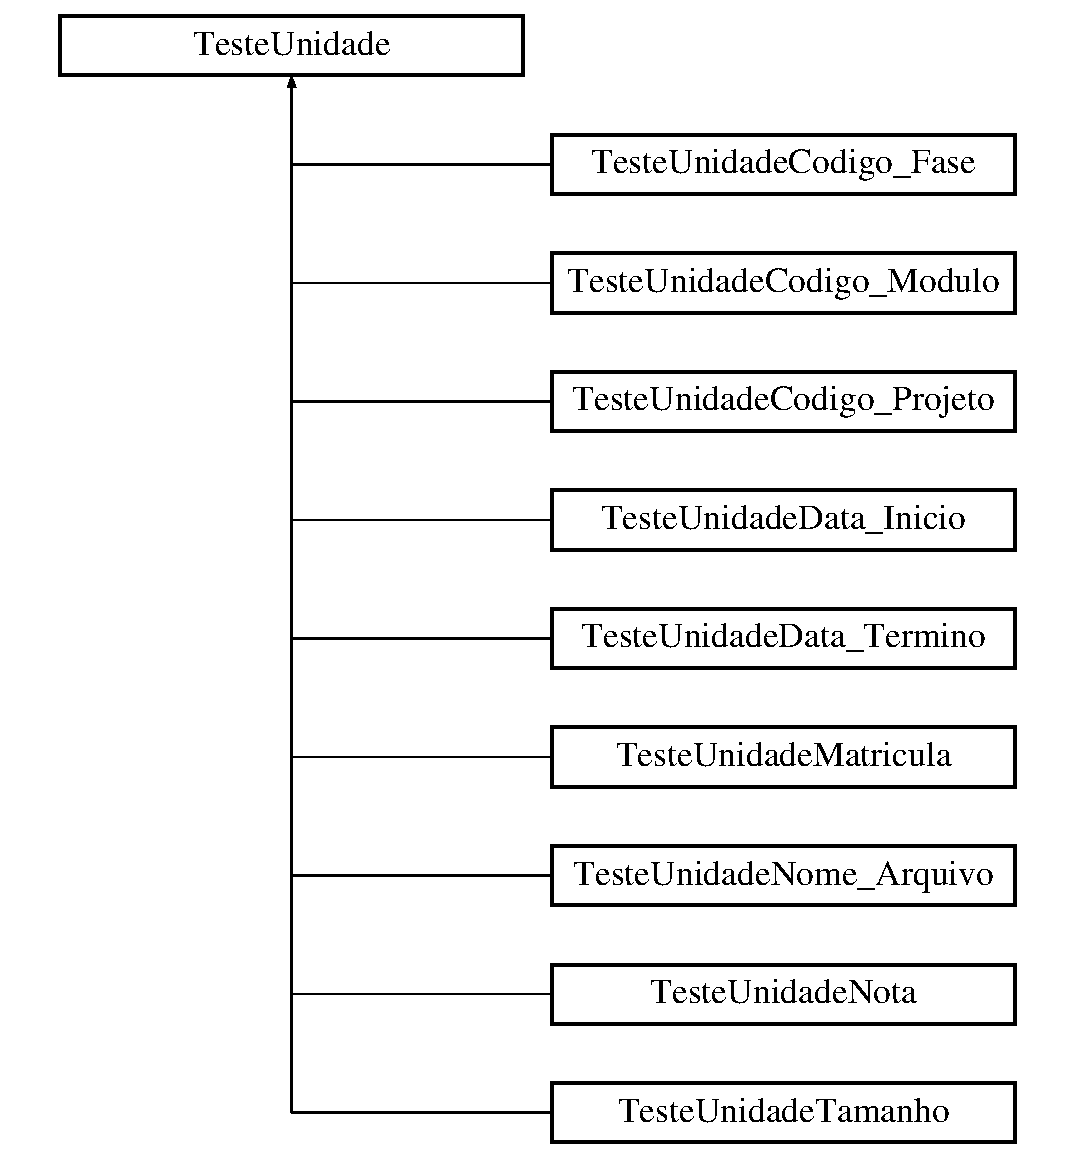
\includegraphics[height=10.000000cm]{class_teste_unidade}
\end{center}
\end{figure}
\subsection*{\-Métodos \-Públicos}
\begin{DoxyCompactItemize}
\item 
\hypertarget{class_teste_unidade_a3d7d79d4ecc0b14cc90f1248de551553}{
virtual void {\bfseries set\-Up} ()=0}
\label{class_teste_unidade_a3d7d79d4ecc0b14cc90f1248de551553}

\item 
\hypertarget{class_teste_unidade_a578b38ccb4674170236280c8786f3eb2}{
virtual void {\bfseries tear\-Down} ()=0}
\label{class_teste_unidade_a578b38ccb4674170236280c8786f3eb2}

\item 
\hypertarget{class_teste_unidade_a6b167d0c3937b54e6e4f1f8616324aab}{
virtual void {\bfseries run} ()=0}
\label{class_teste_unidade_a6b167d0c3937b54e6e4f1f8616324aab}

\end{DoxyCompactItemize}


\subsection{\-Descrição \-Detalhada}
\-Classe \hyperlink{class_teste_unidade}{\-Teste\-Unidade}. 

\-Classe basica para realizacao dos testes 

\-A documentação para esta classe foi gerada a partir do seguinte arquivo\-:\begin{DoxyCompactItemize}
\item 
testestipos.\-h\end{DoxyCompactItemize}

\hypertarget{class_teste_unidade_codigo___fase}{
\section{\-Referência da \-Classe \-Teste\-Unidade\-Codigo\-\_\-\-Fase}
\label{class_teste_unidade_codigo___fase}\index{\-Teste\-Unidade\-Codigo\-\_\-\-Fase@{\-Teste\-Unidade\-Codigo\-\_\-\-Fase}}
}


\-Classe \hyperlink{class_teste_unidade_codigo___fase}{\-Teste\-Unidade\-Codigo\-\_\-\-Fase}.  




{\ttfamily \#include $<$testestipos.\-h$>$}

\-Diagrama de \-Hierarquia para \-Teste\-Unidade\-Codigo\-\_\-\-Fase\-:\begin{figure}[H]
\begin{center}
\leavevmode
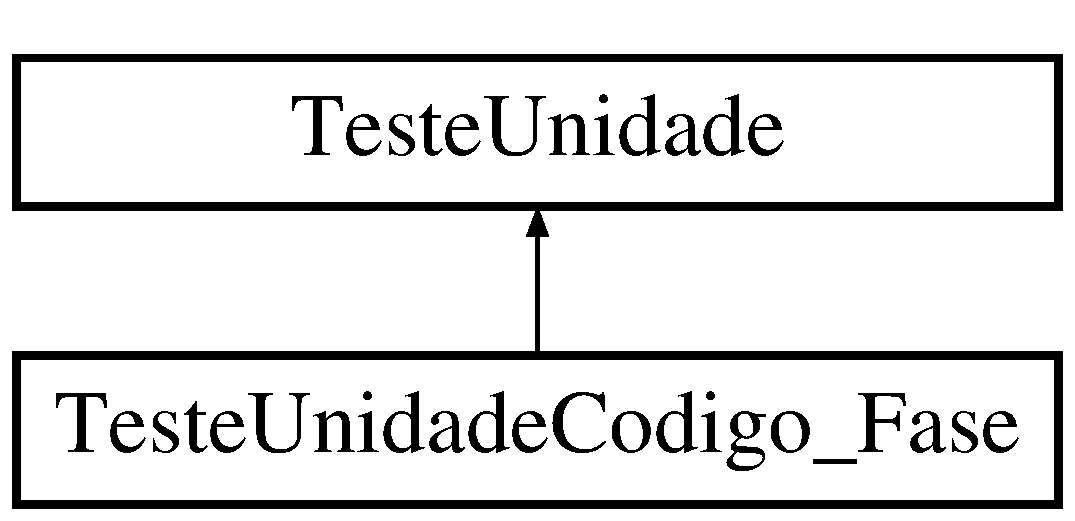
\includegraphics[height=2.000000cm]{class_teste_unidade_codigo___fase}
\end{center}
\end{figure}
\subsection*{\-Métodos \-Públicos}
\begin{DoxyCompactItemize}
\item 
\hypertarget{class_teste_unidade_codigo___fase_a7c3ee4cd4096b53c8640659f098e2053}{
void \hyperlink{class_teste_unidade_codigo___fase_a7c3ee4cd4096b53c8640659f098e2053}{set\-Up} ()}
\label{class_teste_unidade_codigo___fase_a7c3ee4cd4096b53c8640659f098e2053}

\begin{DoxyCompactList}\small\item\em cria uma instancia da classe \-Codigo\-\_\-\-Fase \end{DoxyCompactList}\item 
\hypertarget{class_teste_unidade_codigo___fase_acea7843e220309aab2ef6baf014a15dd}{
void \hyperlink{class_teste_unidade_codigo___fase_acea7843e220309aab2ef6baf014a15dd}{tear\-Down} ()}
\label{class_teste_unidade_codigo___fase_acea7843e220309aab2ef6baf014a15dd}

\begin{DoxyCompactList}\small\item\em deleta a instancia da classe \-Codigo\-\_\-\-Fase \end{DoxyCompactList}\item 
\hypertarget{class_teste_unidade_codigo___fase_a4d4bb33015750352e358c34312e9b55f}{
void \hyperlink{class_teste_unidade_codigo___fase_a4d4bb33015750352e358c34312e9b55f}{run} ()}
\label{class_teste_unidade_codigo___fase_a4d4bb33015750352e358c34312e9b55f}

\begin{DoxyCompactList}\small\item\em executa o \hyperlink{class_teste_unidade_codigo___fase_a7c3ee4cd4096b53c8640659f098e2053}{set\-Up()}, testar\-Valido() , testar\-Invalido(), \hyperlink{class_teste_unidade_codigo___fase_acea7843e220309aab2ef6baf014a15dd}{tear\-Down()}. \end{DoxyCompactList}\end{DoxyCompactItemize}


\subsection{\-Descrição \-Detalhada}
\-Classe \hyperlink{class_teste_unidade_codigo___fase}{\-Teste\-Unidade\-Codigo\-\_\-\-Fase}. 

\-Realiza o teste de validez da classe \-Codigo\-\_\-\-Fase 

\-A documentação para esta classe foi gerada a partir dos seguintes arquivos\-:\begin{DoxyCompactItemize}
\item 
testestipos.\-h\item 
testestipos.\-cpp\end{DoxyCompactItemize}

\hypertarget{class_teste_unidade_codigo___modulo}{
\section{\-Referência da \-Classe \-Teste\-Unidade\-Codigo\-\_\-\-Modulo}
\label{class_teste_unidade_codigo___modulo}\index{\-Teste\-Unidade\-Codigo\-\_\-\-Modulo@{\-Teste\-Unidade\-Codigo\-\_\-\-Modulo}}
}


\-Classe \hyperlink{class_teste_unidade_codigo___modulo}{\-Teste\-Unidade\-Codigo\-\_\-\-Modulo}.  




{\ttfamily \#include $<$testestipos.\-h$>$}

\-Diagrama de \-Hierarquia para \-Teste\-Unidade\-Codigo\-\_\-\-Modulo\-:\begin{figure}[H]
\begin{center}
\leavevmode
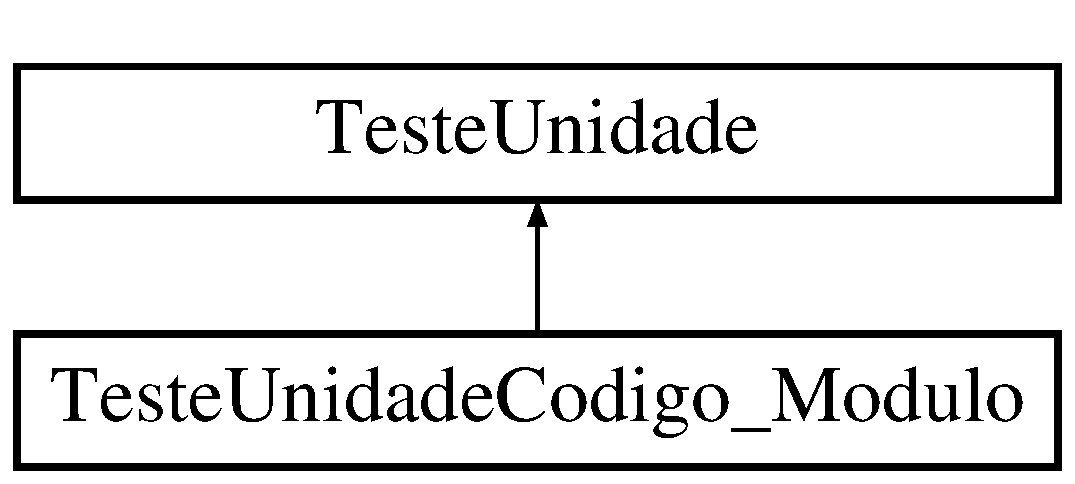
\includegraphics[height=2.000000cm]{class_teste_unidade_codigo___modulo}
\end{center}
\end{figure}
\subsection*{\-Métodos \-Públicos}
\begin{DoxyCompactItemize}
\item 
\hypertarget{class_teste_unidade_codigo___modulo_ab9a7debd6cebfe5708b4f46d3e09878f}{
void \hyperlink{class_teste_unidade_codigo___modulo_ab9a7debd6cebfe5708b4f46d3e09878f}{set\-Up} ()}
\label{class_teste_unidade_codigo___modulo_ab9a7debd6cebfe5708b4f46d3e09878f}

\begin{DoxyCompactList}\small\item\em cria uma instancia da classe \-Codigo\-\_\-\-Modulo \end{DoxyCompactList}\item 
\hypertarget{class_teste_unidade_codigo___modulo_ac5663f6baabc9d3743d227d98d854f2d}{
void \hyperlink{class_teste_unidade_codigo___modulo_ac5663f6baabc9d3743d227d98d854f2d}{tear\-Down} ()}
\label{class_teste_unidade_codigo___modulo_ac5663f6baabc9d3743d227d98d854f2d}

\begin{DoxyCompactList}\small\item\em deleta a instancia da classe \-Codigo\-\_\-\-Modulo \end{DoxyCompactList}\item 
\hypertarget{class_teste_unidade_codigo___modulo_ab56267182e8bc291e100ac9acc0ef562}{
void \hyperlink{class_teste_unidade_codigo___modulo_ab56267182e8bc291e100ac9acc0ef562}{run} ()}
\label{class_teste_unidade_codigo___modulo_ab56267182e8bc291e100ac9acc0ef562}

\begin{DoxyCompactList}\small\item\em executa o \hyperlink{class_teste_unidade_codigo___modulo_ab9a7debd6cebfe5708b4f46d3e09878f}{set\-Up()}, testar\-Valido() , testar\-Invalido(), \hyperlink{class_teste_unidade_codigo___modulo_ac5663f6baabc9d3743d227d98d854f2d}{tear\-Down()}. \end{DoxyCompactList}\end{DoxyCompactItemize}


\subsection{\-Descrição \-Detalhada}
\-Classe \hyperlink{class_teste_unidade_codigo___modulo}{\-Teste\-Unidade\-Codigo\-\_\-\-Modulo}. 

\-Realiza o teste de validez da classe \-Codigo\-\_\-\-Modulo 

\-A documentação para esta classe foi gerada a partir dos seguintes arquivos\-:\begin{DoxyCompactItemize}
\item 
testestipos.\-h\item 
testestipos.\-cpp\end{DoxyCompactItemize}

\hypertarget{class_teste_unidade_codigo___projeto}{
\section{\-Referência da \-Classe \-Teste\-Unidade\-Codigo\-\_\-\-Projeto}
\label{class_teste_unidade_codigo___projeto}\index{\-Teste\-Unidade\-Codigo\-\_\-\-Projeto@{\-Teste\-Unidade\-Codigo\-\_\-\-Projeto}}
}


\-Classe \hyperlink{class_teste_unidade_codigo___projeto}{\-Teste\-Unidade\-Codigo\-\_\-\-Projeto}.  




{\ttfamily \#include $<$testestipos.\-h$>$}

\-Diagrama de \-Hierarquia para \-Teste\-Unidade\-Codigo\-\_\-\-Projeto\-:\begin{figure}[H]
\begin{center}
\leavevmode
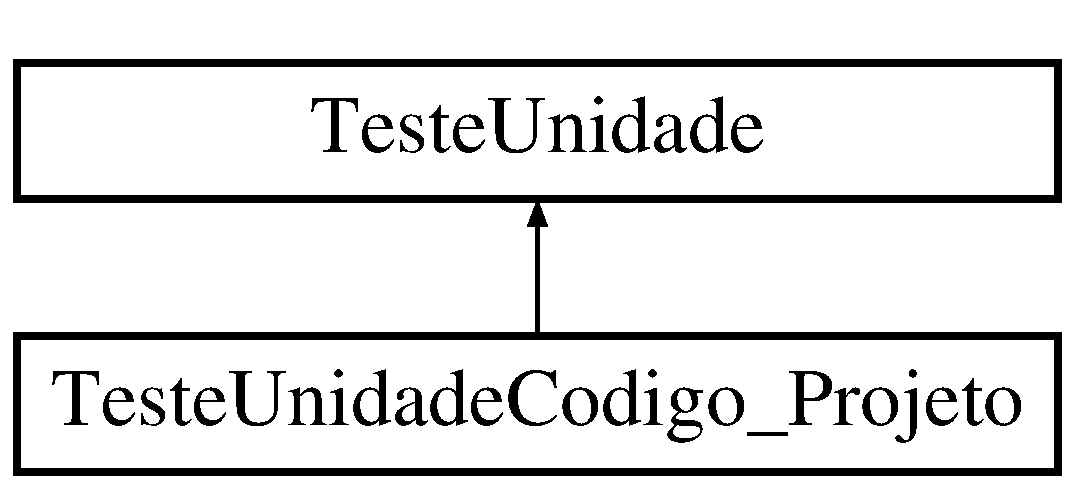
\includegraphics[height=2.000000cm]{class_teste_unidade_codigo___projeto}
\end{center}
\end{figure}
\subsection*{\-Métodos \-Públicos}
\begin{DoxyCompactItemize}
\item 
\hypertarget{class_teste_unidade_codigo___projeto_a08873edf78ee0550b0377da24fc574fb}{
void \hyperlink{class_teste_unidade_codigo___projeto_a08873edf78ee0550b0377da24fc574fb}{set\-Up} ()}
\label{class_teste_unidade_codigo___projeto_a08873edf78ee0550b0377da24fc574fb}

\begin{DoxyCompactList}\small\item\em cria uma instancia da classe \-Codigo\-\_\-\-Projeto \end{DoxyCompactList}\item 
\hypertarget{class_teste_unidade_codigo___projeto_a1e02a73686fa764e0189a24b1b3a5f46}{
void \hyperlink{class_teste_unidade_codigo___projeto_a1e02a73686fa764e0189a24b1b3a5f46}{tear\-Down} ()}
\label{class_teste_unidade_codigo___projeto_a1e02a73686fa764e0189a24b1b3a5f46}

\begin{DoxyCompactList}\small\item\em deleta a instancia da classe \-Codigo\-\_\-\-Projeto \end{DoxyCompactList}\item 
\hypertarget{class_teste_unidade_codigo___projeto_ab54dceaedb9cc4bbd14360b97d6a47a3}{
void \hyperlink{class_teste_unidade_codigo___projeto_ab54dceaedb9cc4bbd14360b97d6a47a3}{run} ()}
\label{class_teste_unidade_codigo___projeto_ab54dceaedb9cc4bbd14360b97d6a47a3}

\begin{DoxyCompactList}\small\item\em executa o \hyperlink{class_teste_unidade_codigo___projeto_a08873edf78ee0550b0377da24fc574fb}{set\-Up()}, testar\-Valido() , testar\-Invalido(), \hyperlink{class_teste_unidade_codigo___projeto_a1e02a73686fa764e0189a24b1b3a5f46}{tear\-Down()}. \end{DoxyCompactList}\end{DoxyCompactItemize}


\subsection{\-Descrição \-Detalhada}
\-Classe \hyperlink{class_teste_unidade_codigo___projeto}{\-Teste\-Unidade\-Codigo\-\_\-\-Projeto}. 

\-Realiza o teste de validez da classe \-Codigo\-\_\-\-Projeto 

\-A documentação para esta classe foi gerada a partir dos seguintes arquivos\-:\begin{DoxyCompactItemize}
\item 
testestipos.\-h\item 
testestipos.\-cpp\end{DoxyCompactItemize}

\hypertarget{class_teste_unidade_data___inicio}{
\section{\-Referência da \-Classe \-Teste\-Unidade\-Data\-\_\-\-Inicio}
\label{class_teste_unidade_data___inicio}\index{\-Teste\-Unidade\-Data\-\_\-\-Inicio@{\-Teste\-Unidade\-Data\-\_\-\-Inicio}}
}


\-Classe \hyperlink{class_teste_unidade_data___inicio}{\-Teste\-Unidade\-Data\-\_\-\-Inicio}.  




{\ttfamily \#include $<$testestipos.\-h$>$}

\-Diagrama de \-Hierarquia para \-Teste\-Unidade\-Data\-\_\-\-Inicio\-:\begin{figure}[H]
\begin{center}
\leavevmode
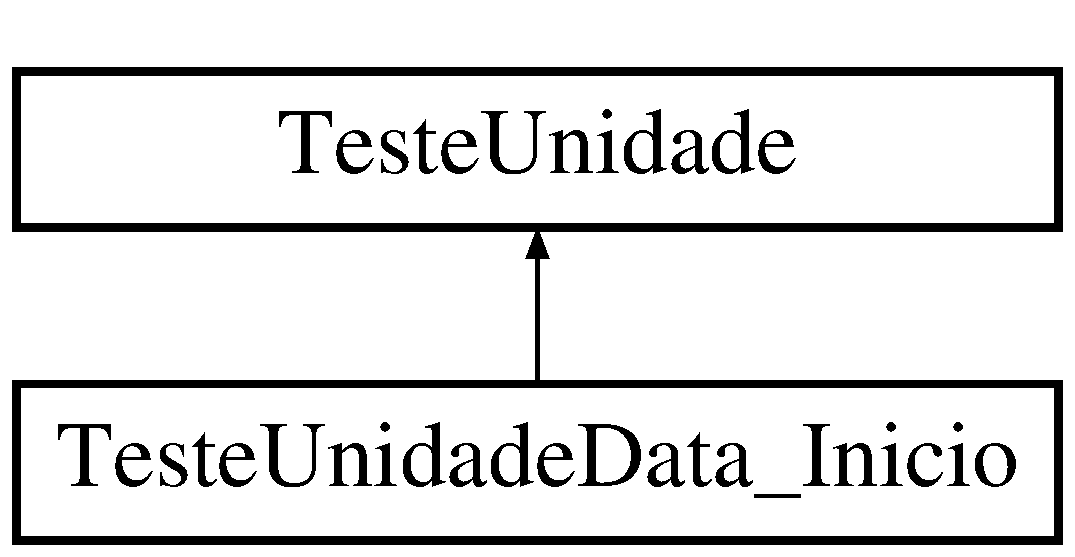
\includegraphics[height=2.000000cm]{class_teste_unidade_data___inicio}
\end{center}
\end{figure}
\subsection*{\-Métodos \-Públicos}
\begin{DoxyCompactItemize}
\item 
\hypertarget{class_teste_unidade_data___inicio_aaddfb2e6b483890801372ab84f05bca2}{
void \hyperlink{class_teste_unidade_data___inicio_aaddfb2e6b483890801372ab84f05bca2}{set\-Up} ()}
\label{class_teste_unidade_data___inicio_aaddfb2e6b483890801372ab84f05bca2}

\begin{DoxyCompactList}\small\item\em cria uma instancia da classe \-Data\-\_\-\-Inicio \end{DoxyCompactList}\item 
\hypertarget{class_teste_unidade_data___inicio_a7f1e225037892bbc000bb492ac7a739f}{
void \hyperlink{class_teste_unidade_data___inicio_a7f1e225037892bbc000bb492ac7a739f}{tear\-Down} ()}
\label{class_teste_unidade_data___inicio_a7f1e225037892bbc000bb492ac7a739f}

\begin{DoxyCompactList}\small\item\em deleta a instancia da classe \-Data\-\_\-\-Inicio \end{DoxyCompactList}\item 
\hypertarget{class_teste_unidade_data___inicio_a9f86daa2f2c6807f91f77719b0ef7a0d}{
void \hyperlink{class_teste_unidade_data___inicio_a9f86daa2f2c6807f91f77719b0ef7a0d}{run} ()}
\label{class_teste_unidade_data___inicio_a9f86daa2f2c6807f91f77719b0ef7a0d}

\begin{DoxyCompactList}\small\item\em executa o \hyperlink{class_teste_unidade_data___inicio_aaddfb2e6b483890801372ab84f05bca2}{set\-Up()}, testar\-Valido() , testar\-Invalido(), \hyperlink{class_teste_unidade_data___inicio_a7f1e225037892bbc000bb492ac7a739f}{tear\-Down()}. \end{DoxyCompactList}\end{DoxyCompactItemize}


\subsection{\-Descrição \-Detalhada}
\-Classe \hyperlink{class_teste_unidade_data___inicio}{\-Teste\-Unidade\-Data\-\_\-\-Inicio}. 

\-Realiza o teste de validez da classe \-Data\-\_\-\-Inicio 

\-A documentação para esta classe foi gerada a partir dos seguintes arquivos\-:\begin{DoxyCompactItemize}
\item 
testestipos.\-h\item 
testestipos.\-cpp\end{DoxyCompactItemize}

\hypertarget{class_teste_unidade_data___termino}{
\section{\-Referência da \-Classe \-Teste\-Unidade\-Data\-\_\-\-Termino}
\label{class_teste_unidade_data___termino}\index{\-Teste\-Unidade\-Data\-\_\-\-Termino@{\-Teste\-Unidade\-Data\-\_\-\-Termino}}
}


\-Classe \hyperlink{class_teste_unidade_data___termino}{\-Teste\-Unidade\-Data\-\_\-\-Termino}.  




{\ttfamily \#include $<$testestipos.\-h$>$}

\-Diagrama de \-Hierarquia para \-Teste\-Unidade\-Data\-\_\-\-Termino\-:\begin{figure}[H]
\begin{center}
\leavevmode
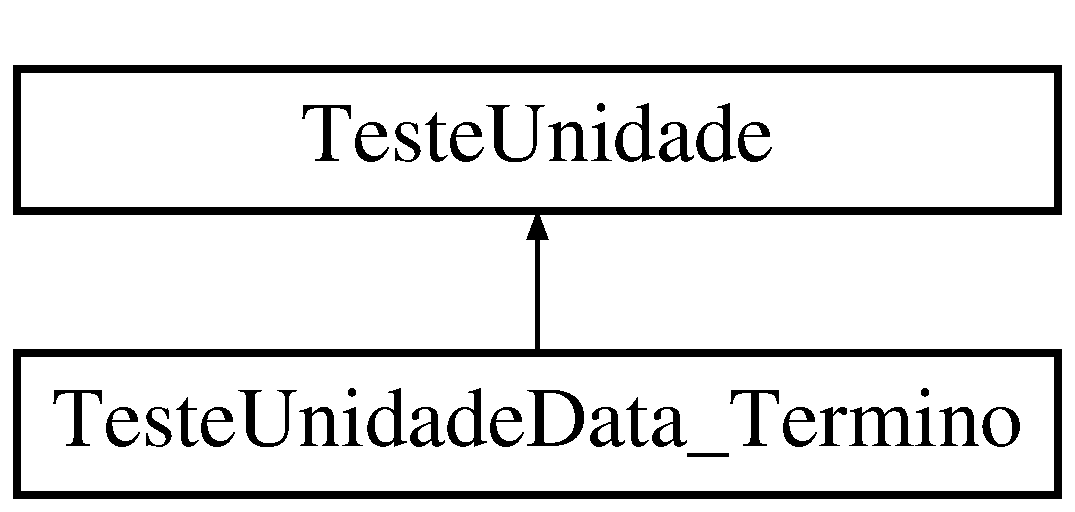
\includegraphics[height=2.000000cm]{class_teste_unidade_data___termino}
\end{center}
\end{figure}
\subsection*{\-Métodos \-Públicos}
\begin{DoxyCompactItemize}
\item 
\hypertarget{class_teste_unidade_data___termino_a0c6693f95f1b90b068e2cab6c9889662}{
void \hyperlink{class_teste_unidade_data___termino_a0c6693f95f1b90b068e2cab6c9889662}{set\-Up} ()}
\label{class_teste_unidade_data___termino_a0c6693f95f1b90b068e2cab6c9889662}

\begin{DoxyCompactList}\small\item\em cria uma instancia da classe \-Data\-\_\-\-Termino \end{DoxyCompactList}\item 
\hypertarget{class_teste_unidade_data___termino_a02bc5c95c16c1de7dcfd63f9d59e36d3}{
void \hyperlink{class_teste_unidade_data___termino_a02bc5c95c16c1de7dcfd63f9d59e36d3}{tear\-Down} ()}
\label{class_teste_unidade_data___termino_a02bc5c95c16c1de7dcfd63f9d59e36d3}

\begin{DoxyCompactList}\small\item\em deleta a instancia da classe \-Data\-\_\-\-Termino \end{DoxyCompactList}\item 
\hypertarget{class_teste_unidade_data___termino_a9c59cd926ba305c855ed5e476445e6f4}{
void \hyperlink{class_teste_unidade_data___termino_a9c59cd926ba305c855ed5e476445e6f4}{run} ()}
\label{class_teste_unidade_data___termino_a9c59cd926ba305c855ed5e476445e6f4}

\begin{DoxyCompactList}\small\item\em executa o \hyperlink{class_teste_unidade_data___termino_a0c6693f95f1b90b068e2cab6c9889662}{set\-Up()}, testar\-Valido() , testar\-Invalido(), \hyperlink{class_teste_unidade_data___termino_a02bc5c95c16c1de7dcfd63f9d59e36d3}{tear\-Down()}. \end{DoxyCompactList}\end{DoxyCompactItemize}


\subsection{\-Descrição \-Detalhada}
\-Classe \hyperlink{class_teste_unidade_data___termino}{\-Teste\-Unidade\-Data\-\_\-\-Termino}. 

\-Realiza o teste de validez da classe \-Data\-\_\-\-Termino 

\-A documentação para esta classe foi gerada a partir dos seguintes arquivos\-:\begin{DoxyCompactItemize}
\item 
testestipos.\-h\item 
testestipos.\-cpp\end{DoxyCompactItemize}

\hypertarget{class_teste_unidade_matricula}{
\section{\-Referência da \-Classe \-Teste\-Unidade\-Matricula}
\label{class_teste_unidade_matricula}\index{\-Teste\-Unidade\-Matricula@{\-Teste\-Unidade\-Matricula}}
}


\-Classe \hyperlink{class_teste_unidade_matricula}{\-Teste\-Unidade\-Matricula}.  




{\ttfamily \#include $<$testestipos.\-h$>$}

\-Diagrama de \-Hierarquia para \-Teste\-Unidade\-Matricula\-:\begin{figure}[H]
\begin{center}
\leavevmode
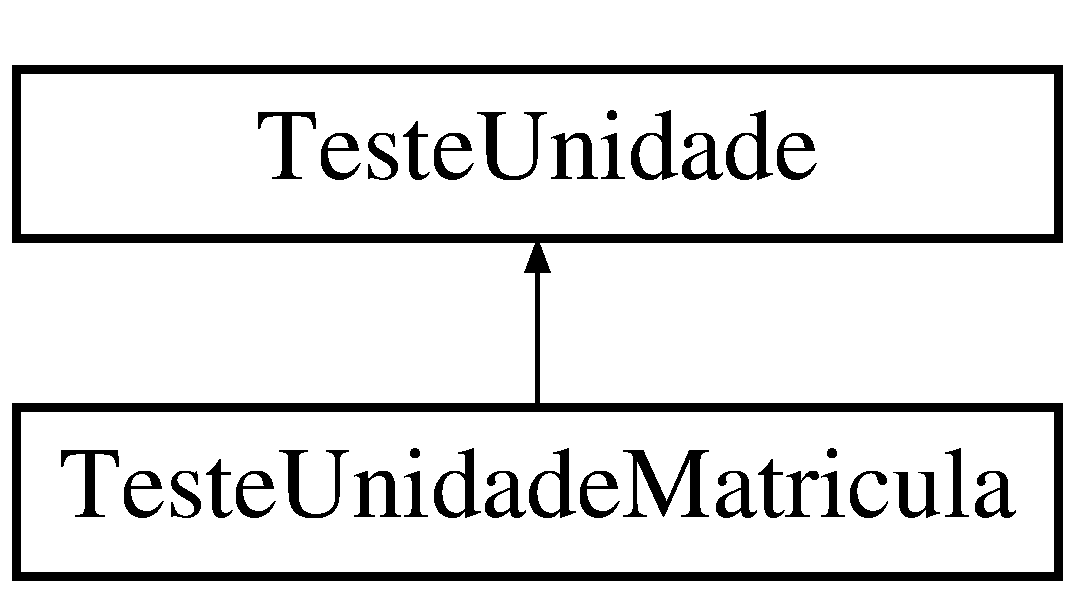
\includegraphics[height=2.000000cm]{class_teste_unidade_matricula}
\end{center}
\end{figure}
\subsection*{\-Métodos \-Públicos}
\begin{DoxyCompactItemize}
\item 
\hypertarget{class_teste_unidade_matricula_aa5289b85d9097a5cd776889066a2a21e}{
void \hyperlink{class_teste_unidade_matricula_aa5289b85d9097a5cd776889066a2a21e}{set\-Up} ()}
\label{class_teste_unidade_matricula_aa5289b85d9097a5cd776889066a2a21e}

\begin{DoxyCompactList}\small\item\em cria uma instancia da classe \-Matricula \end{DoxyCompactList}\item 
\hypertarget{class_teste_unidade_matricula_acd40e1914bdfb2eaddc1e24dcda6a92d}{
void \hyperlink{class_teste_unidade_matricula_acd40e1914bdfb2eaddc1e24dcda6a92d}{tear\-Down} ()}
\label{class_teste_unidade_matricula_acd40e1914bdfb2eaddc1e24dcda6a92d}

\begin{DoxyCompactList}\small\item\em deleta a instancia da classe \-Matricula \end{DoxyCompactList}\item 
\hypertarget{class_teste_unidade_matricula_af9494e1ba911d9f8a84df252057f4fd7}{
void \hyperlink{class_teste_unidade_matricula_af9494e1ba911d9f8a84df252057f4fd7}{run} ()}
\label{class_teste_unidade_matricula_af9494e1ba911d9f8a84df252057f4fd7}

\begin{DoxyCompactList}\small\item\em executa o \hyperlink{class_teste_unidade_matricula_aa5289b85d9097a5cd776889066a2a21e}{set\-Up()}, testar\-Valido() , testar\-Invalido(), \hyperlink{class_teste_unidade_matricula_acd40e1914bdfb2eaddc1e24dcda6a92d}{tear\-Down()}. \end{DoxyCompactList}\end{DoxyCompactItemize}


\subsection{\-Descrição \-Detalhada}
\-Classe \hyperlink{class_teste_unidade_matricula}{\-Teste\-Unidade\-Matricula}. 

\-Realiza o teste de validez da classe \-Matricula 

\-A documentação para esta classe foi gerada a partir dos seguintes arquivos\-:\begin{DoxyCompactItemize}
\item 
testestipos.\-h\item 
testestipos.\-cpp\end{DoxyCompactItemize}

\hypertarget{class_teste_unidade_nome___arquivo}{
\section{\-Referência da \-Classe \-Teste\-Unidade\-Nome\-\_\-\-Arquivo}
\label{class_teste_unidade_nome___arquivo}\index{\-Teste\-Unidade\-Nome\-\_\-\-Arquivo@{\-Teste\-Unidade\-Nome\-\_\-\-Arquivo}}
}


\-Classe \hyperlink{class_teste_unidade_nome___arquivo}{\-Teste\-Unidade\-Nome\-\_\-\-Arquivo}.  




{\ttfamily \#include $<$testestipos.\-h$>$}

\-Diagrama de \-Hierarquia para \-Teste\-Unidade\-Nome\-\_\-\-Arquivo\-:\begin{figure}[H]
\begin{center}
\leavevmode
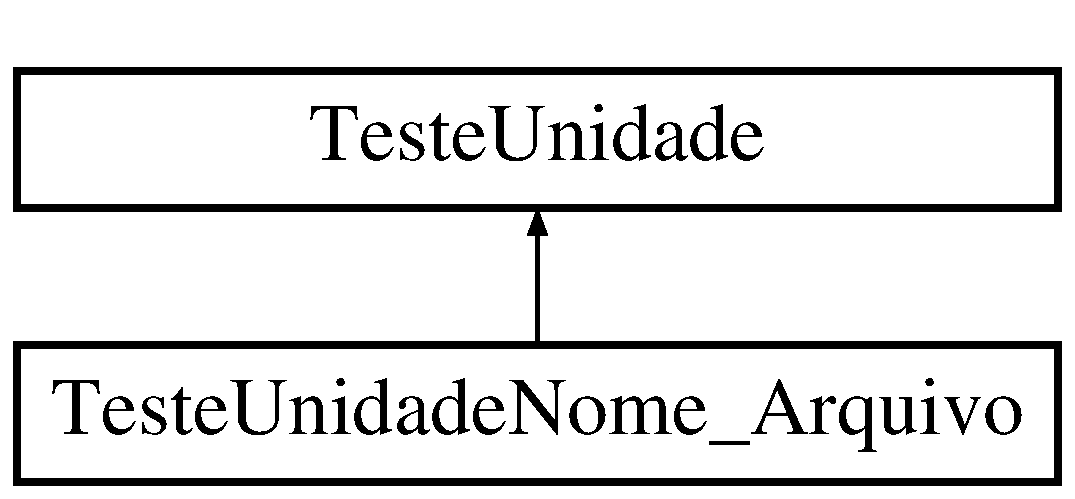
\includegraphics[height=2.000000cm]{class_teste_unidade_nome___arquivo}
\end{center}
\end{figure}
\subsection*{\-Métodos \-Públicos}
\begin{DoxyCompactItemize}
\item 
\hypertarget{class_teste_unidade_nome___arquivo_a796f85778140f739fe2e6e8e1f87b731}{
void \hyperlink{class_teste_unidade_nome___arquivo_a796f85778140f739fe2e6e8e1f87b731}{set\-Up} ()}
\label{class_teste_unidade_nome___arquivo_a796f85778140f739fe2e6e8e1f87b731}

\begin{DoxyCompactList}\small\item\em cria uma instancia da classe \-Nome\-\_\-\-Arquivo \end{DoxyCompactList}\item 
\hypertarget{class_teste_unidade_nome___arquivo_a2626213ef3c457d3956c058d522cf34a}{
void \hyperlink{class_teste_unidade_nome___arquivo_a2626213ef3c457d3956c058d522cf34a}{tear\-Down} ()}
\label{class_teste_unidade_nome___arquivo_a2626213ef3c457d3956c058d522cf34a}

\begin{DoxyCompactList}\small\item\em deleta a instancia da classe \-Nome\-\_\-\-Arquivo \end{DoxyCompactList}\item 
\hypertarget{class_teste_unidade_nome___arquivo_a4e6ee79dcbde8c2b2ff5ca6b6a990335}{
void \hyperlink{class_teste_unidade_nome___arquivo_a4e6ee79dcbde8c2b2ff5ca6b6a990335}{run} ()}
\label{class_teste_unidade_nome___arquivo_a4e6ee79dcbde8c2b2ff5ca6b6a990335}

\begin{DoxyCompactList}\small\item\em executa o \hyperlink{class_teste_unidade_nome___arquivo_a796f85778140f739fe2e6e8e1f87b731}{set\-Up()}, testar\-Valido() , testar\-Invalido(), \hyperlink{class_teste_unidade_nome___arquivo_a2626213ef3c457d3956c058d522cf34a}{tear\-Down()}. \end{DoxyCompactList}\end{DoxyCompactItemize}


\subsection{\-Descrição \-Detalhada}
\-Classe \hyperlink{class_teste_unidade_nome___arquivo}{\-Teste\-Unidade\-Nome\-\_\-\-Arquivo}. 

\-Realiza o teste de validez da classe \-Nome\-\_\-\-Arquivo 

\-A documentação para esta classe foi gerada a partir dos seguintes arquivos\-:\begin{DoxyCompactItemize}
\item 
testestipos.\-h\item 
testestipos.\-cpp\end{DoxyCompactItemize}

\hypertarget{class_teste_unidade_nota}{
\section{\-Referência da \-Classe \-Teste\-Unidade\-Nota}
\label{class_teste_unidade_nota}\index{\-Teste\-Unidade\-Nota@{\-Teste\-Unidade\-Nota}}
}


\-Classe \hyperlink{class_teste_unidade_nota}{\-Teste\-Unidade\-Nota}.  




{\ttfamily \#include $<$testestipos.\-h$>$}

\-Diagrama de \-Hierarquia para \-Teste\-Unidade\-Nota\-:\begin{figure}[H]
\begin{center}
\leavevmode
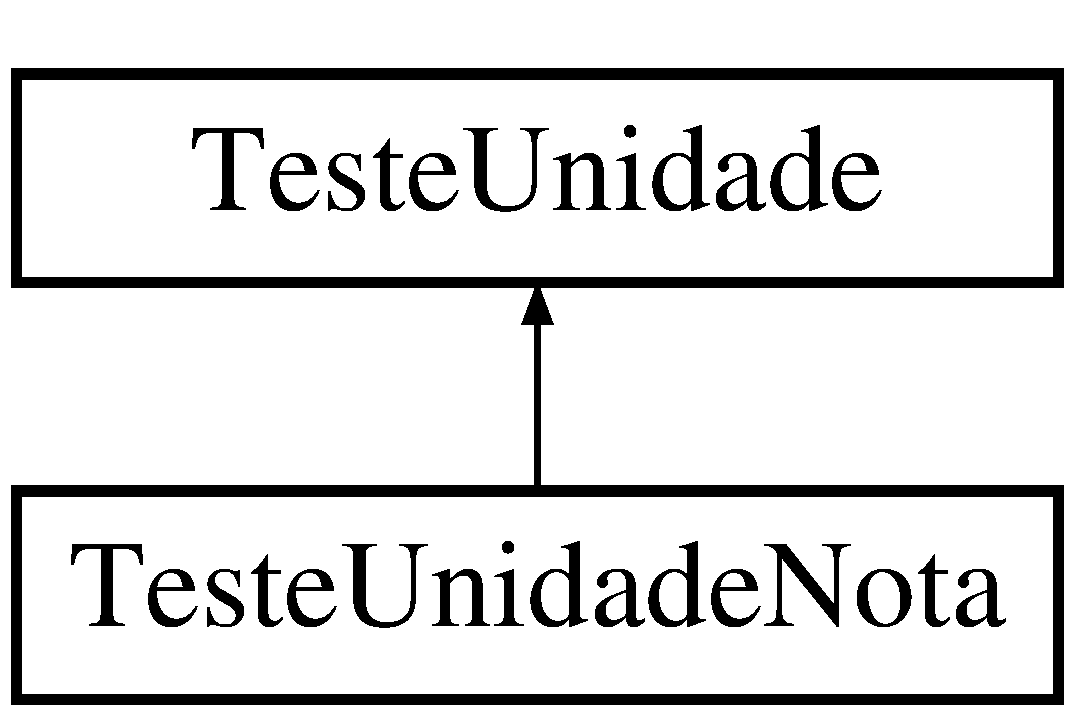
\includegraphics[height=2.000000cm]{class_teste_unidade_nota}
\end{center}
\end{figure}
\subsection*{\-Métodos \-Públicos}
\begin{DoxyCompactItemize}
\item 
\hypertarget{class_teste_unidade_nota_a152acba800d4faff31e1f4a8b9126c4b}{
void \hyperlink{class_teste_unidade_nota_a152acba800d4faff31e1f4a8b9126c4b}{set\-Up} ()}
\label{class_teste_unidade_nota_a152acba800d4faff31e1f4a8b9126c4b}

\begin{DoxyCompactList}\small\item\em cria uma instancia da classe \-Nota \end{DoxyCompactList}\item 
\hypertarget{class_teste_unidade_nota_a13e06cf32e7c61b3db4849b26a2c2926}{
void \hyperlink{class_teste_unidade_nota_a13e06cf32e7c61b3db4849b26a2c2926}{tear\-Down} ()}
\label{class_teste_unidade_nota_a13e06cf32e7c61b3db4849b26a2c2926}

\begin{DoxyCompactList}\small\item\em deleta a instancia da classe \-Nota \end{DoxyCompactList}\item 
\hypertarget{class_teste_unidade_nota_a7364d87fd0c80a9b2064a76eaea8b923}{
void \hyperlink{class_teste_unidade_nota_a7364d87fd0c80a9b2064a76eaea8b923}{run} ()}
\label{class_teste_unidade_nota_a7364d87fd0c80a9b2064a76eaea8b923}

\begin{DoxyCompactList}\small\item\em executa o \hyperlink{class_teste_unidade_nota_a152acba800d4faff31e1f4a8b9126c4b}{set\-Up()}, testar\-Valido() , testar\-Invalido(), \hyperlink{class_teste_unidade_nota_a13e06cf32e7c61b3db4849b26a2c2926}{tear\-Down()}. \end{DoxyCompactList}\end{DoxyCompactItemize}


\subsection{\-Descrição \-Detalhada}
\-Classe \hyperlink{class_teste_unidade_nota}{\-Teste\-Unidade\-Nota}. 

\-Realiza o teste de validez da classe \-Nota 

\-A documentação para esta classe foi gerada a partir dos seguintes arquivos\-:\begin{DoxyCompactItemize}
\item 
testestipos.\-h\item 
testestipos.\-cpp\end{DoxyCompactItemize}

\hypertarget{class_teste_unidade_tamanho}{
\section{\-Referência da \-Classe \-Teste\-Unidade\-Tamanho}
\label{class_teste_unidade_tamanho}\index{\-Teste\-Unidade\-Tamanho@{\-Teste\-Unidade\-Tamanho}}
}


\-Classe \hyperlink{class_teste_unidade_tamanho}{\-Teste\-Unidade\-Tamanho}.  




{\ttfamily \#include $<$testestipos.\-h$>$}

\-Diagrama de \-Hierarquia para \-Teste\-Unidade\-Tamanho\-:\begin{figure}[H]
\begin{center}
\leavevmode
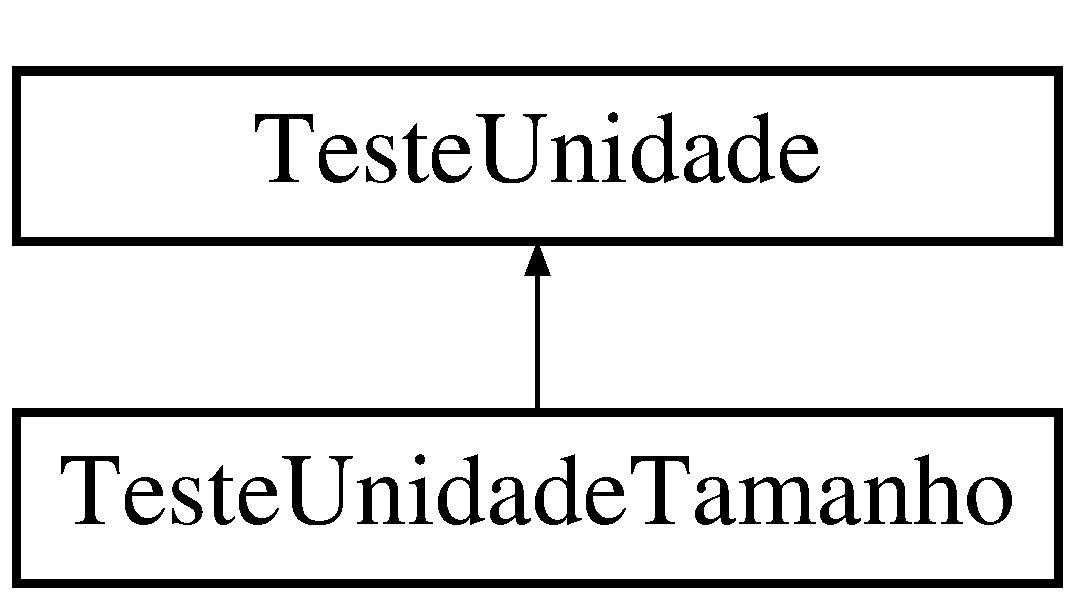
\includegraphics[height=2.000000cm]{class_teste_unidade_tamanho}
\end{center}
\end{figure}
\subsection*{\-Métodos \-Públicos}
\begin{DoxyCompactItemize}
\item 
\hypertarget{class_teste_unidade_tamanho_aadca7a2934b8832990a48cbe55ee832b}{
void \hyperlink{class_teste_unidade_tamanho_aadca7a2934b8832990a48cbe55ee832b}{set\-Up} ()}
\label{class_teste_unidade_tamanho_aadca7a2934b8832990a48cbe55ee832b}

\begin{DoxyCompactList}\small\item\em cria uma instancia da classe \-Tamanho \end{DoxyCompactList}\item 
\hypertarget{class_teste_unidade_tamanho_a63cadec089bb5bc16dc9978084260fc8}{
void \hyperlink{class_teste_unidade_tamanho_a63cadec089bb5bc16dc9978084260fc8}{tear\-Down} ()}
\label{class_teste_unidade_tamanho_a63cadec089bb5bc16dc9978084260fc8}

\begin{DoxyCompactList}\small\item\em deleta a instancia da classe \-Tamanho \end{DoxyCompactList}\item 
\hypertarget{class_teste_unidade_tamanho_af9bb3a26b5efeafd92798e2eefd91151}{
void \hyperlink{class_teste_unidade_tamanho_af9bb3a26b5efeafd92798e2eefd91151}{run} ()}
\label{class_teste_unidade_tamanho_af9bb3a26b5efeafd92798e2eefd91151}

\begin{DoxyCompactList}\small\item\em executa o \hyperlink{class_teste_unidade_tamanho_aadca7a2934b8832990a48cbe55ee832b}{set\-Up()}, testar\-Valido() , testar\-Invalido(), \hyperlink{class_teste_unidade_tamanho_a63cadec089bb5bc16dc9978084260fc8}{tear\-Down()}. \end{DoxyCompactList}\end{DoxyCompactItemize}


\subsection{\-Descrição \-Detalhada}
\-Classe \hyperlink{class_teste_unidade_tamanho}{\-Teste\-Unidade\-Tamanho}. 

\-Realiza o teste de validez da classe \-Tamanho 

\-A documentação para esta classe foi gerada a partir dos seguintes arquivos\-:\begin{DoxyCompactItemize}
\item 
testestipos.\-h\item 
testestipos.\-cpp\end{DoxyCompactItemize}

\printindex
\end{document}
